\chapter{Literature Review}
\label{ch:literature_review}

We performed a literature review regarding distributed reinforcement learning,
and categorized the results according to groups of tags.
This review was made with the purpose of highlighting recent trends in distributed RL and frequently used algorithms, RL metrics,
and relevant system and network communication benchmarks.
To gather relevant literature, we searched the Web of Science database using the following search query,
while limiting the results to the last 5 years:

\begin{verbatim}
    ALL=
    (
        (
            "distributed" OR "parallel" OR
            "multi-agent" OR "asynchronous"
        )
        AND
        (
            "shared environments" OR "replay buffer" OR
            "trajectory sampling" OR "experience sampling"
        )
        AND "reinforcement learning"
    )
\end{verbatim}

Initially, a total of 68 papers matched the search query, with 34 being deemed irrelevant to the
present research question or lacking sufficient scientific validity.
The remaining 33 references were analyzed, and tagged according to the following categories:

\begin{itemize}[leftmargin=*, label={--}]
    \item \textbf{Algorithm Categories} (e.g., Q-learning, Actor-Critic, Policy Gradients)
    \item \textbf{Learning Paradigm} (On-Policy, Off-Policy, Model-Free, Model-Based)
    \item \textbf{Communication Model} (Centralized, Decentralized, Asynchronous, Synchronous)
    \item \textbf{RL Metrics} (Reward, Sample Efficiency, Convergence, Stability)
    \item \textbf{System Metrics} (Wall Speed, Latency, Memory, Core Efficiency)
\end{itemize}

\section{Algorithmic Landscape}
\label{sec:algorithmic-landscape}

The algorithm categories analyzed, as shown in \cref{fig:algorithm}, revealed a clear preference for actor-critic architectures (6 out of 33 papers),
followed by Q-learning variants including DQN and DDPG (4), and to a lesser extent SAC, PPO, and Impala.
Only one paper made use of Gorila, despite its historical role in scaling Q-learning via distributed experience replay.
This reflects a general trend toward architectures that decouple policy evaluation from improvement—either via off-policy learning or multithreaded experience collection.
The diversity suggests no one-size-fits-all solution, but rather that algorithmic selection is often tailored to the resource constraints and task structure at hand.

\begin{figure}
    \centering
    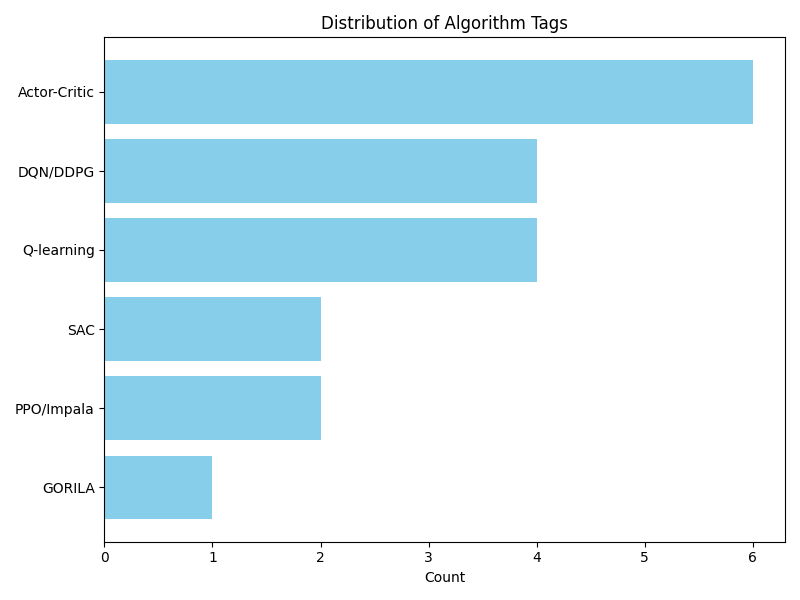
\includegraphics[width=0.8\textwidth]{images/literature/algorithm}
    \caption{Algorithm classes}
    \label{fig:algorithm}
\end{figure}

\section{Communication Models and Scalability}
\label{sec:communication-models-and-scalability}

Decentralized architectures were most frequent for our search query (8 instances), often favored for scalability and fault tolerance.
Centralized (5) and asynchronous (5) methods are frequently used in systems where shared state must be maintained across learners,
with synchronous designs being less common, shown in \cref{fig:communication_type}.
The prevalence of asynchronous and decentralized schemes underscores the challenge of balancing policy staleness with communication overhead
—a trade-off directly addressed in designs like IMPALA and SEED RL.

\begin{figure}
    \centering
    \includegraphics[width=0.8\textwidth]{images/literature/communication}
    \caption{Communication type}
    \label{fig:communication_type}
\end{figure}

\section{RL and Performance Metrics}
\label{sec:rl-and-performance-metrics}

Among RL-specific evaluation criteria, convergence and sample efficiency dominate (8 and 7 mentions respectively),
highlighting the central importance of rapid learning and stable policy improvement, as shown in \cref{fig:rl_metrics}.
Stability and reward-related scores are also commonly used (6 each), though reward alone is rarely sufficient to benchmark system improvements in distributed settings.
The frequent attention to convergence and efficiency metrics reflects a growing awareness that communication overhead and resource utilization can significantly
impact learning dynamics, particularly in systems with many concurrent agents.

Tagged system metrics are shown in \cref{fig:system_metrics}.
Wall time (7), memory usage (5), and latency (5) are frequently reported, with core efficiency trailing slightly (4).
These metrics are crucial when deploying RL systems in performance-sensitive environments like financial markets or real-time robotics.
Wall time, often used as a proxy for overall training throughput, receives particular attention,
emphasizing care put in reducing time-to-solution.
This aligns with our own motivation for optimizing PEARL to accommodate the throughput demands of high-frequency trading environments.

\begin{figure}[htbp]
    \centering
    \begin{minipage}[t]{0.48\textwidth}
        \centering
        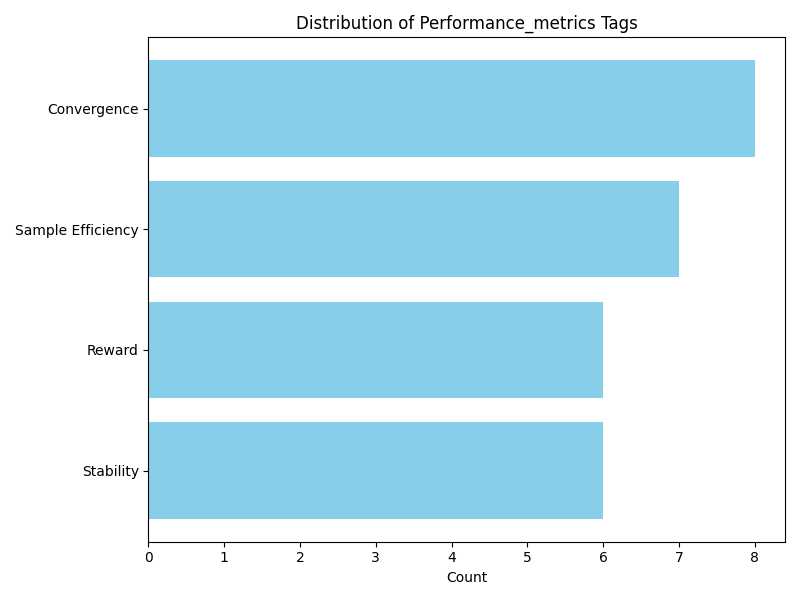
\includegraphics[width=\textwidth]{images/literature/rl_metrics}
        \caption{Reinforcement learning-based metrics}
        \label{fig:rl_metrics}
    \end{minipage}
    \hfill
    \begin{minipage}[t]{0.48\textwidth}
        \centering
        \includegraphics[width=\textwidth]{images/literature/system_metrics}
        \caption{System and network metrics}
        \label{fig:system_metrics}
    \end{minipage}
\end{figure}

\section{Conclusion of the Literature Review}
\label{sec:conclusion-of-the-literature-review}

Overall, the literature points to a growing interest in modular, scalable, and \textbf{asynchronous architectures} that can adapt to diverse computational environments,
while still maintaining acceptable training speeds and sample efficiency.
\textbf{Actor-Critic} methods, particularly those employing off-policy or asynchronous updates, dominate the field due to their flexibility and \textbf{sample efficiency}.
Communication remains a central bottleneck, with decentralization and batching strategies like those used in SEED RL emerging as practical solutions.

Building on these insights, we introduce PEARL, a system designed for \textbf{multi-agent reinforcement learning}, where
timing, throughput, and low-latency responses are critical, such as financial simulations.
The architecture, designed to minimize inter-process communication,
is based on a \textbf{parallel asynchronous} interface between learners and shared environments.
In the following sections, we discuss the system's implementation details,
and evaluate its performance in terms of wall time, latency, core efficiency and training reward.